\documentclass[12pt]{article}
\usepackage[utf8]{inputenc}
\usepackage{amsmath}
\usepackage{soul}
\usepackage{xcolor}
\usepackage{amssymb}
\usepackage{float}
\usepackage{graphicx}
\usepackage{geometry}
\usepackage{framed} % For the box
\sethlcolor{yellow}
\newcommand{\red}[1]{\textcolor{red}{#1}}
\newcommand{\blue}[1]{\textcolor{blue}{#1}}

% Adjust margins
\geometry{margin=1in}

\title{\textbf{CSE421: Design and Analysis of Algorithms}}
\author{Homework 1 \\ Shaqan Oveis Gharan}
\date{March 27th, 2024 \\ Due: April 3rd, 2024 at 11:59 PM}


\begin{document}

\noindent CS-3510-\textbf{\red{Your Section\#}} Algorithms, Spring 2025\hfill Mid-Term 1 Take-Home\\
\blue{FirstName} \blue{LastName} \hfill Collaborator(s):

\hrulefill

\subsection*{Problem 1 (10 pts)}
For this problem, we explore the issue of \textit{truthfulness} in the Gale-Shapley algorithm for Stable Matching. Show that a participant can improve its outcome by lying about its preferences. Consider $r \in R$. Suppose $r$ prefers $p$ to $p'$, but $p$ and $p'$ are low on $r$'s preference list. Show that it is possible that by switching the order of $p$ and $p'$ on $r$'s preference list, $r$ achieves a better outcome, e.g., is matched with a $p''$ higher on the preference list than the one if the actual order was used.

\textit{Hint:} Prove the claim by finding one specific instance of stable matching problem and comparing the stable matching before and after the switching.

\subsection*{Solution}

We can show that it is possible for a receiver $r$ to obtain a more-preferred match by being untruthful, by switching the order of two options that $r$ actually likes less (even though in his true ranking one is better than the other).

Let the two sides be:
\begin{itemize}
    \item \textbf{Residents (receivers)} $R$: $r, s, t$
    \item \textbf{Programs (proposers)} $P$: $p, p', q$
\end{itemize}
Assume that the matching is produced by a \textbf{program-proposing Gale-Shapley algorithm}.

\subsubsection*{True Preference Lists}
\begin{itemize}
    \item \textbf{Resident $r$'s true preferences:}  
    \[
    q > p > p'
    \]
    So $r$ likes $q$ best; although he prefers $p$ to $p'$, both $p$ and $p'$ are lower than $q$.

    \item \textbf{Resident $s$'s true preferences:}  
    \[
    p > q > p'
    \]

    \item \textbf{Resident $t$'s true preferences:}  
    \[
    p > p' > q
    \]

    \item \textbf{Programs' preferences:}
    \begin{itemize}
        \item $p$: $r > s > t$
        \item $p'$: $r > t > s$
        \item $q$: $s > r > t$
    \end{itemize}
\end{itemize}

\subsubsection*{Outcome When $r$ Reports Truthfully}
We run the \textbf{program-proposing Gale-Shapley algorithm} using the true lists.

\begin{enumerate}
    \item \textbf{Round 1:}
    \begin{itemize}
        \item $p$ proposes to its top choice: $r$.
        \item $p'$ also proposes to its top choice: $r$.
        \item $q$ proposes to its top choice: $s$.
    \end{itemize}

    \item \textbf{Resident Decisions:}
    \begin{itemize}
        \item $r$ receives proposals from $p$ and $p'$.
        \item Using his true order $q > p > p'$, he compares these two. Since $p > p'$ in his true list, he tentatively holds $p$ and rejects $p'$.
        \item $s$ gets $q$.
        \item $t$ gets no proposal in this round.
    \end{itemize}

    \item \textbf{Round 2:}
    \begin{itemize}
        \item $p'$, having been rejected by $r$, now moves to its next choice and proposes to $t$.
    \end{itemize}

    \item \textbf{Final Matching:}
    \begin{itemize}
        \item $r$ is matched with $p$.
        \item $s$ is matched with $q$.
        \item $t$ is matched with $p'$.
    \end{itemize}
\end{enumerate}

Outcome for $r$: He gets $p$, but he would prefer $q$ over $p$. Since $q$ proposed only to $s$, $q$ is already taken.

\subsubsection*{Outcome When $r$ Misreports}
Now suppose that $r$ lies about his 2nd and 3rd rankings by switching $p$ and $p'$. In other words, he submits as his preference list:
\[
q > p' > p
\]
Even though he actually prefers $p$ to $p'$, he reverses these when reporting.

Now run the algorithm again:

\begin{enumerate}
    \item \textbf{Round 1:}
    \begin{itemize}
        \item $p$ proposes to its top choice: $r$.
        \item $p'$ proposes to its top choice: $r$.
        \item $q$ proposes to its top choice: $s$.
    \end{itemize}

    \item \textbf{Resident Decisions:}
    \begin{itemize}
        \item $r$ receives proposals from $p$ and $p'$.  
        \item Using his reported order $q > p' > p$, he compares the two proposals and holds $p'$ (since $p' > p$ in his reported list), rejecting $p$.
        \item $s$ gets $q$.
        \item $t$ gets nothing yet.
    \end{itemize}

    \item \textbf{Round 2:}
    \begin{itemize}
        \item $p$, having been rejected by $r$, moves to its next choice and proposes to $s$.
        \item $s$'s true order is $p > q > p'$, so she prefers $p$ over $q$.
        \item $s$ drops $q$ and holds $p$.
        \item $q$, now rejected by $s$, proposes to its next choice, which is $r$.
    \end{itemize}

    \item \textbf{Round 3:}
    \begin{itemize}
        \item $r$ is currently holding $p'$ from round 1.
        \item Now $r$ receives a proposal from $q$.
        \item Since $r$'s true order is $q > p > p'$, he prefers $q$ over his current match $p'$.
        \item So $r$ drops $p'$ and accepts $q$.
    \end{itemize}

    \item \textbf{Round 4:}
    \begin{itemize}
        \item $p'$, now rejected by $r$, goes to its next choice and proposes to $t$.
        \item $t$ (true order: $p > p' > q$) accepts $p'$.
    \end{itemize}

    \item \textbf{Final Matching:}
    \begin{itemize}
        \item $r$ is now matched with $q$.
        \item $s$ is matched with $p$.
        \item $t$ is matched with $p'$.
    \end{itemize}
\end{enumerate}

\subsubsection*{Conclusion}
By simply swapping the order of $p$ and $p'$ in his reported preference list (even though he truly prefers $p$ to $p'$), resident $r$ can trigger a different chain reaction of proposals. 

In the truthful run, he ended up with $p$ (his second choice). However, by lying, he eventually receives a proposal from $q$, his true first choice. 

This proves that in the program-proposing Gale-Shapley algorithm, truth-telling is not necessarily an optimal strategy. A participant can benefit by misreporting their preferences.

\subsection*{Problem 2 (10 pts)}
Arrange in increasing order of asymptotic growth. All logs are in base 2.

\begin{enumerate}
    \item \( n^{\frac{5}{3}} \log^2 n \)
    \item \( 2^{\sqrt{\log n}} \)
    \item \( \sqrt{n^n} \)
    \item \( \frac{n^2}{\log n} \)
    \item \( 2^n \)
\end{enumerate}

\subsection*{Solution}

We want to compare the asymptotic growth of five functions as \(n \to \infty\):

\[
f_1(n) = n^{\tfrac{5}{3}} (\log n)^2, 
\quad
f_2(n) = 2^{\sqrt{\log n}}, 
\quad
f_3(n) = \sqrt{n^n} = n^{\tfrac{n}{2}}, 
\quad
f_4(n) = \frac{n^2}{\log n},
\quad
f_5(n) = 2^n.
\]

\subsubsection*{Step 1: Comparing \(f_2(n)\) with polynomials}
First, compare \(f_2(n) = 2^{\sqrt{\log n}}\) to polynomial functions of \(n\). 

Note that 
\[
\log_2 \bigl( 2^{\sqrt{\log_2 n}} \bigr) 
= \sqrt{\log_2 n},
\quad
\log_2 \bigl(n^x \bigr)
= x \log_2 n.
\]
As \(n \to \infty\), \(x \log_2 n\) (linear in \(\log_2 n\)) will outgrow \(\sqrt{\log_2 n}\). Therefore
\[
2^{\sqrt{\log n}} = 2^{\sqrt{\log_2 n}} 
\; < \; 
n^x
\quad
\text{for any fixed } x > 0.
\]
Because \(f_1(n) = n^{5/3} (\log n)^2\) and \(f_4(n) = \tfrac{n^2}{\log n}\) are both polynomial, we can conclude
\[
f_2(n) \; < \; f_1(n), 
\quad
f_2(n) \; < \; f_4(n).
\]

\subsubsection*{Step 2: Comparing \(f_1(n)\) and \(f_4(n)\)}
Next, compare
\[
f_1(n) = n^{\tfrac{5}{3}} (\log n)^2
\quad\text{and}\quad
f_4(n) = \frac{n^2}{\log n}.
\]
Examine their ratio:
\[
\frac{f_1(n)}{f_4(n)}
= \frac{n^{\tfrac{5}{3}} \,(\log n)^2}{\tfrac{n^2}{\log n}}
= \frac{n^{\tfrac{5}{3}} (\log n)^3}{n^2}
= \frac{(\log n)^3}{n^{\tfrac{1}{3}}}.
\]
Since \(n^{\tfrac{1}{3}}\) outgrows \((\log n)^3\) as \(n\to\infty\), we have 
\(\tfrac{(\log n)^3}{n^{1/3}} \to 0\). Thus
\[
f_1(n) \; < \; f_4(n).
\]

So far, we have
\[
f_2(n) \; < \; f_1(n) \; < \; f_4(n).
\]

\subsubsection*{Step 3: Comparing the exponentials \(f_3(n)\) vs.\ \(f_5(n)\)}
Finally, compare
\[
f_3(n) = n^{\tfrac{n}{2}},
\quad 
f_5(n) = 2^n.
\]
Rewrite them as exponentials:
\[
f_3(n) = \exp\Bigl(\tfrac{n}{2} \ln n\Bigr),
\quad
f_5(n) = \exp\bigl(n \ln 2\bigr).
\]
Compare their exponents:
\[
\tfrac{n}{2} \ln n
\quad \text{vs.} \quad
n \ln 2.
\]
Since \(\ln n\) grows unbounded, eventually \(\tfrac{1}{2}\ln n\) exceeds \(\ln 2\), so
\[
\tfrac{n}{2} \ln n 
\;\gg\;
n \ln 2.
\]
Hence 
\[
n^{\tfrac{n}{2}} 
\;\gg\;
2^n,
\]
meaning \(f_3(n)\) grows faster than \(f_5(n)\).

\subsubsection*{Step 4: Final Ordering}
Combining all comparisons, the increasing order of asymptotic growth is:
\[
\boxed{
2^{\sqrt{\log n}} 
\;<\; 
n^{\tfrac{5}{3}} (\log n)^2 
\;<\; 
\frac{n^2}{\log n} 
\;<\; 
2^n 
\;<\; 
\sqrt{n^n}\,.
}
\]

\subsection*{Problem 3 (10 pts)}
We say that $T(n)$ is $O(f(n))$ if there exist $c$ and $n_0$ such that for all $n > n_0,\:T(n) \le cf(n)$. Use this definition for parts $a$ and $b$.
\begin{enumerate}
    \item Prove that $4n^2 + 3n\text{log}\:n + 6n + 20\text{log}^2n + 11$ is $O(n^2)$. (You may use, without proof, the fact that $\text{log}\:n < n$ for $n \ge 1$.)
    \item Suppose that $f(n)$ is $O(r(n))$ and $g(n)$ is $O(s(n))$. Let $h(n) = f(n)g(n)$ and $t(n) = r(n)s(n)$. Prove that $h(n)$ is $O(t(n))$.
\end{enumerate}

\subsection*{Solution}

\subsubsection*{(a) Proof that $4n^2 + 3n\text{log}\:n + 6n + 20\text{log}^2n + 11$ is $O(n^2)$.}

Let
\[
T(n) \;=\; 4n^2 \;+\; 3n \log n \;+\; 6n \;+\; 20 (\log n)^2 \;+\; 11.
\]
We want to prove that $T(n) = O(n^2)$. We bound each term separately:
\begin{itemize}
\item $4n^2$ is obviously $O(n^2)$.
\item Since $\log n < n$ for $n \ge 1$, $3n \log n < 3n^2$.
\item For $n \ge 1$, $6n < 6n^2$.
\item For large $n$, $(\log n)^2 < n^2$, so $20(\log n)^2 < 20n^2$.
\item For $n \ge 1$, $11 \le 11n^2$.
\end{itemize}
Each of these bounds is at most $O(n^2)$.
Therefore, $T(n)$ is $O(n^2)$.

\subsubsection*{(b) Proof that $h(n)$ is $O(t(n))$.}

Assume $f(n)$ is $O(r(n))$ and $g(n)$ is $O(s(n))$. By definition, there exist constants $c_1, c_2 > 0$ and $n_1, n_2$ such that
\[
f(n) \;\le\; c_1\,r(n) \quad \text{for all } n > n_1,
\quad\text{and}\quad
g(n) \;\le\; c_2\,s(n) \quad \text{for all } n > n_2.
\]
Let $n_0 = \max\{n_1,\,n_2\}$. Then for $n > n_0$, we have
\[
f(n)\,g(n)
\;\le\;
\bigl(c_1\,r(n)\bigr)\,\bigl(c_2\,s(n)\bigr)
\;=\;
c_1\,c_2\;\bigl(r(n)\,s(n)\bigr).
\]
Since $c_1 c_2$ is just another constant, this shows
\[
f(n)\,g(n) = O\bigl(r(n)\,s(n)\bigr).
\]

\subsection*{Problem 4 (10 pts)}
The \textit{diameter} of an undirected graph is the maximum distance between any pair of vertices. If a graph is not connected, its diameter is infinite. Let $G$ be an $n$ node undirected graph, where $n$ is even. Suppose that every vertex has degree at least n/2. Prove that G has diameter at most 2.

\textit{Hint:} Proof by contradiction

\subsection*{Problem 5 (10 pts)}
Show that there are at least $3\cdot2^{n-1}$ ways to properly color vertices of a tree T with n vertices using 3 colors, i.e., to color vertices with three colors such that any two adjacent vertices have  distinct colors. Note that it can be shown that there are exactly $3\cdot2^{n-1}$ ways to properly color vertices of T with 3 colors but in this problem, to receive full credit, it is enough prove the “at least” part.\\
For example, there are (at least) $3\cdot2^2 = 12$ ways to color a tree with 3 vertices as show below:

\begin{figure}[H]
    \centering
    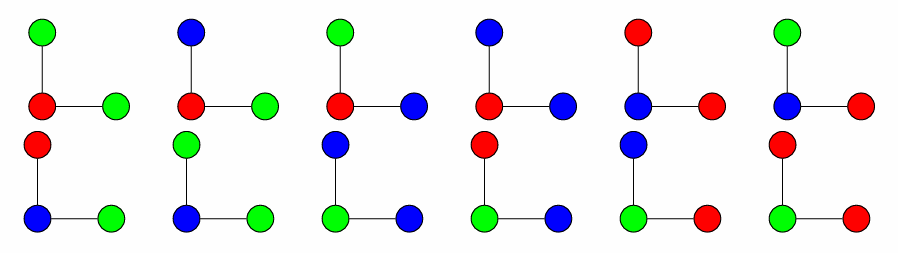
\includegraphics[width=0.8\linewidth]{P5.png}
    \label{fig:3-color-graph}
\end{figure}

\subsection*{Problem 6 (Extra Credit: 10 pts)}
Given a directed graph $G$ with $n$ vertices $V = \{1,2,\cdots,n\}$ and $m$ edges. We say that a vertex $j$ is reachable from $i$ if there is a directed path from $i$ to $j$. Design an $O(m+n)$-time algorithm (show the pseudo-code) that for any vertex $i$ outputs the smallest label reachable from $i$. For example, given the following graph you should output 1,2,2,2,1 corresponding to the smallest indices reachable from vertices 1,2,3,4,5 respectively.
\begin{figure}[H]
    \centering
    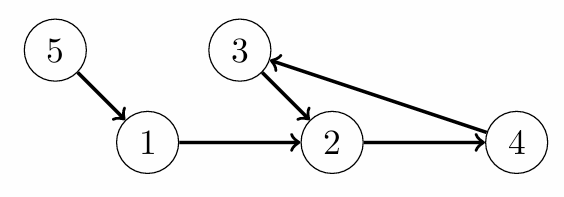
\includegraphics[width=0.5\linewidth]{P6.png}
    \label{fig:P6}
\end{figure}

\end{document}


